% paper-agent paper — IEEE conference format
% Build: paper-agent compile paper/main.tex   (latexmk -pdf, output in paper/build/)
\documentclass[conference]{IEEEtran}
\IEEEoverridecommandlockouts

\usepackage[utf8]{inputenc}
\usepackage[T1]{fontenc}
\usepackage{cite}
\usepackage{amsmath,amssymb,amsfonts}
\usepackage{graphicx}
\usepackage{booktabs}
\usepackage{array}
\usepackage{xcolor}
\usepackage{url}
\usepackage[hidelinks]{hyperref}
\usepackage{microtype}

\graphicspath{{figures/}}

% \todo{} marks items that must be resolved before submission
\newcommand{\todo}[1]{\textcolor{red}{[TODO: #1]}}
% placeholder token as it appears in the masked text, e.g. \ph{3}
\newcommand{\ph}[1]{\texttt{[[#1]]}}

\begin{document}

\title{Which Model Actually Answered? Silent Model Substitution, Deterministic Validators, and Multi-Model Routing in an LLM Paper Agent}

\author{%
\IEEEauthorblockN{Andi Agung Dwi Arya B}
\IEEEauthorblockA{\textit{Program Studi Magister Teknik Informatika, Fakultas Teknik} \\
\textit{Universitas Hasanuddin}\\
Makassar, Indonesia \\
D082251054 $\cdot$ \todo{email}}
}

\maketitle

\begin{abstract}
Research agents increasingly call commercial large language models (LLMs) through vendor SDKs and report the model name they requested as the provenance of their output. We show that this label can be wrong: the vendor's CLI accepts any model name and, when the account is not entitled to it, silently serves a different model---Claude Opus 4.8 was requested and Claude Haiku 4.5 answered, and a fictitious model name ``succeeded'' as well. Only the provider's usage event names the model that answered. We build this observation into \emph{paper-agent}, an open-source agent for scientific papers that (i) records the served model of every call, (ii) routes work to models by role, and (iii) wraps every model output in deterministic validators. Its structure-safe translation masks LaTeX into placeholders and emphasis tags whose multiset and number-gluing are verified per unit. On an eight-section IEEE paper (146 units, 4{,}673 words, 262 placeholders) we compare a three-model pipeline (draft, post-edit by a different model, back-translation QA by a local model, per-unit selection) with two single-model configurations. The pipeline and the single API model both keep all 146 units structurally intact (the local model loses two); the pipeline's glossary compliance (99.0\%) and mean cross-lingual cosine (0.826 direct, 0.958 back-translation) are \emph{not} higher than those of the single model (99.7\%; 0.837, 0.961), and it costs three times the wall time. Its value is error catching: a sentence left in English, a wrong technical term, and placeholders moved in front of numbers were found only because a second model re-read the text and because validators rejected malformed output. Three error classes---moved placeholders, a QA model that echoed its input, and dropped placeholders---were detected by no model, including the judge, but by the validators. We argue that served-model provenance and deterministic validation should be standard in research agents, and that multi-model review is best applied selectively.
\end{abstract}


\begin{IEEEkeywords}
large language models, model routing, provenance, machine translation, LaTeX, compound AI systems, LLM-as-a-judge, research agents
\end{IEEEkeywords}

\section{Introduction}
\label{sec:intro}

Scientific software built around LLMs is now routinely a \emph{compound} system: several models, retrieval components and rule-based checks cooperate, and the choice of model per step is a design variable rather than a constant~\cite{chen2024compound,chen2023frugalgpt,ong2024routellm}. Research agents that read, translate, review or summarise papers are a prominent case, and their results enter theses and publications together with a statement of the kind ``the LLM was \texttt{model-X}''. That statement is part of the scientific record: it decides whether a result can be reproduced and whether two runs are comparable.

This paper starts from an incident in such a system. A neuro-symbolic agent for detecting synthesis-gap indicators in scientific literature~\cite{arya2026wizard} called a commercial model through the GitHub Copilot SDK~\cite{copilotsdk2026} and labelled every result with the configured model, \texttt{claude-opus-4.8-fast}. When the account's entitlement changed, the CLI kept accepting the name---and kept returning answers---while a different model, \texttt{claude-haiku-4.5}, was doing the work. Nothing in the response signalled the substitution; a fictitious model name was accepted just as quietly. The only reliable evidence was a usage event that names the model that answered. The label in the thesis was, for a period, wrong.

The incident raises a general question for research agents: \emph{which model actually answered, and how should an agent know, record and exploit that?} We turn the question into three research questions.
\begin{itemize}
  \item \textbf{RQ1} Does the model that answers a request equal the model that was requested, and what mechanism gives an agent a truthful provenance label?
  \item \textbf{RQ2} On a structure-sensitive task---translating a LaTeX paper while keeping citations, mathematics and cross-references intact---does a pipeline that combines different models (translator, post-editor, judge) outperform a single model, and at what cost?
  \item \textbf{RQ3} Which errors are caught by models (a second model re-reading the output) and which only by deterministic validators?
\end{itemize}

We answer them with \emph{paper-agent}, an open-source agent for scientific papers whose every LLM call records the model that answered, routes work to models by role, and validates every model output deterministically. The contributions are:
\begin{itemize}
  \item an empirical account of silent model substitution in a vendor SDK and a provenance mechanism (served-model logging, substitution warnings, truthful labels) that we recommend for research agents;
  \item a structure-safe translation method for LaTeX that masks commands, mathematics and references into placeholders and emphasis into tags, verifies their multiset and their attachment to numbers per unit, and reproduces the source byte for byte when no translation is applied;
  \item a controlled comparison of a three-model pipeline with two single-model configurations on the same 146 units, with per-unit metrics (cross-lingual cosine, back-translation cosine, glossary compliance, structural integrity, time, served models) released with the code;
  \item an error analysis showing that the pipeline's benefit lies in catching errors rather than in raising averages, and that three error classes were invisible to every model, including the judge, but caught by validators.
\end{itemize}
The agent also verifies references against bibliographic databases, gates citations, builds and checks the PDF, reviews a paper with two independent critics, and converts Word manuscripts to IEEE LaTeX; these functions are described as part of the system but evaluated only informally here. The Indonesian version of this paper was produced by the agent itself.

\section{Related Work}
\label{sec:related}

\paragraph{Compound systems, routing and ensembles}
FrugalGPT showed that cascading cheap and expensive models can match a strong model at a fraction of the cost~\cite{chen2023frugalgpt}; RouteLLM learns a router from preference data~\cite{ong2024routellm}; LLM-Blender ranks and fuses the outputs of several models~\cite{jiang2023blender}; Mixture-of-Agents layers models that refine each other's answers~\cite{wang2024moa}. Chen et al.\ observe that more calls do not monotonically help and that the benefit depends on the task's difficulty distribution~\cite{chen2024compound}. Our pipeline is a small compound system with fixed roles; our contribution is not a better router but the finding that the combination's value on our task shows up in error catching rather than in mean quality, and that deterministic validators are the component that catches the most.

\paragraph{Models judging models}
LLM-as-a-judge agrees with humans at the level of inter-annotator agreement on chat tasks~\cite{zheng2023judge}, and iterative self-feedback improves many generation tasks~\cite{madaan2023selfrefine,shinn2023reflexion}. Two results caution against a single model judging itself: LLMs cannot reliably self-correct reasoning without external signals~\cite{huang2024selfcorrect}, and LLM evaluators recognise and favour their own generations~\cite{panickssery2024selfpref}. We therefore use a \emph{different} model as post-editor, a third one for back-translation, and never let a model be the sole arbiter of structural validity.

\paragraph{Machine-translation quality estimation}
Reference-based metrics such as COMET~\cite{rei2020comet} need human references we do not have; expert MQM annotation~\cite{freitag2021mqm} is the gold standard but costly. Round-trip translation has been revisited as a reference-free estimator~\cite{moon2020roundtrip}, GPT-class models are competitive translators~\cite{hendy2023gpt} and state-of-the-art translation evaluators~\cite{kocmi2023gemba}. We combine a cross-lingual sentence-embedding similarity~\cite{reimers2019sbert,reimers2020multilingual} with back-translation by a local model~\cite{gemma2025}; back-translation as a technique originates in data augmentation~\cite{sennrich2016backtranslation}. Terminology consistency, enforced in neural MT through constrained decoding~\cite{dinu2019terminology}, is handled here by a glossary in the prompt and measured deterministically afterwards.

\paragraph{Provenance and model documentation}
Model cards~\cite{mitchell2019modelcards} document what a model is; hallucination surveys~\cite{ji2023hallucination} document what it may fabricate. Both presuppose that the system knows which model it is using. Vendor documentation lists which models each subscription tier may use~\cite{githubdocs2026models} and independent leaderboards rank them for research-style tasks~\cite{artificialanalysis2026}, but neither tells a running agent what it was served. ReAct-style agents~\cite{yao2023react} that act on tool results would act on a wrong model label just as readily; we add the served model to the trace.

\section{System Design}
\label{sec:method}

\begin{figure*}[t]
  \centering
  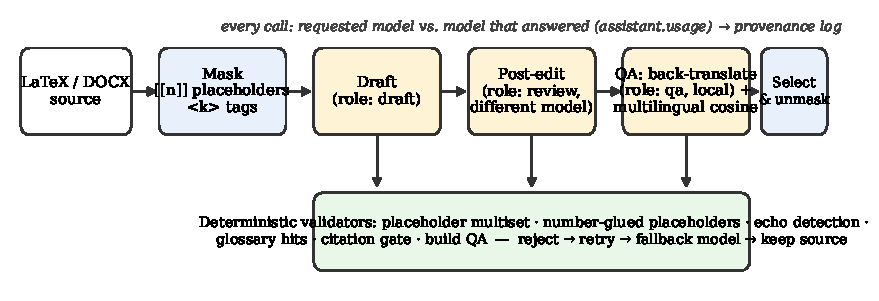
\includegraphics[width=0.92\textwidth]{fig1_architecture.pdf}
  \caption{Structure-safe translation in paper-agent. LaTeX is masked into placeholders and tags; three model roles (draft, post-edit, QA) are filled by different models; deterministic validators sit under every model call and reject malformed output (retry, fallback model, finally keep the source). Every call logs the requested and the served model.}
  \label{fig:arch}
\end{figure*}

Fig.~\ref{fig:arch} shows the translation path of paper-agent; the other commands (reference verification, citation gate, build QA, two-critic review, DOCX conversion, natural-language task planning) share the same engines, roles and provenance log. The agent is a Python package with a command-line interface and an HTTP API; every LLM call goes through one of two engines, a local Ollama server or a commercial SDK~\cite{copilotsdk2026} that fronts Claude and GPT models.

\subsection{Served-Model Provenance}
\label{sec:prov}
The commercial SDK runs the vendor's CLI as a subprocess and exposes a session API. We observed that a session created with any \texttt{model} string answers; when the account is not entitled to the model, another model is used and no error or field in the response indicates it. The session, however, emits an \texttt{assistant.usage} event whose \texttt{model} field names the model that generated the tokens. The engine subscribes to this event for every call, returns the text together with the served model, counts requested and served models separately, and prints a one-time warning per (requested, served) pair. All reports produced by the agent (translation reports, review reports, task-run summaries) carry the served models. The local engine records the model name returned by the server, which is always the requested one.

\subsection{Model Roles}
Work is assigned to \emph{roles}, not to models: \textsc{draft} (translator), \textsc{review} (post-editor), \textsc{qa} (back-translator), \textsc{fallback}, \textsc{critic} and \textsc{critic2} (independent reviewers), \textsc{planner}. The default binding reflects the models an entry-level subscription is entitled to---GPT-5 mini for drafting, Claude Haiku 4.5 for post-editing and critique---plus a local Gemma 3 27B~\cite{gemma2025} for QA, fallback and the second critic; the binding is overridden by an environment variable. Two rules are fixed: the post-editor is never the drafting model, and the two critics are never the same model~\cite{panickssery2024selfpref,huang2024selfcorrect}.

\subsection{Structure-Safe Masking}
\label{sec:mask}
Each line of a LaTeX section file is split into translatable \emph{units}: a paragraph, the argument of \verb|\section|/\verb|\caption|/\verb|\paragraph|, a table cell (the row is split on top-level \verb|&|), or an \verb|\item| body. Lines that are pure structure (\verb|\begin|, \verb|\label|, \verb|\includegraphics|, rules, comments) are kept verbatim. Inside a unit, mathematics (\verb|$...$|), citations, references, labels, identifiers (\verb|\texttt|, \verb|\textsc|), braces groups, \verb|~|, \verb|\%| and every other command with its arguments are replaced by numbered placeholders \ph{n}; adjacent masked spans merge into one placeholder. The emphasis commands \verb|\emph|, \verb|\textbf| and \verb|\textit| become inline tags \verb|<k>...</k>| whose content is still translated. Unmasking reverses both, escapes bare specials the model may have typed (\verb|%|, \verb|&|, \verb|_|), normalises typographic quotes and dashes back to LaTeX, and restores the unit's leading and trailing whitespace. Masking followed by unmasking without translation reproduces every source file byte for byte; this is a unit test and a dry-run check of the tool. A final deterministic pass rewrites the word before \verb|~\ref| (``Fig.'', ``Table'', ``Section'') into the target language, since models occasionally leave it untranslated.

\subsection{Deterministic Validators}
\label{sec:validators}
Every model output for a unit is accepted only if (i) the multiset of placeholders equals that of the source, (ii) the multiset of tags equals that of the source, and (iii) every placeholder that is glued to a number in the source (``58\ph{3}'' standing for \verb|58\%|) is glued to the same number in the output (a decimal comma is tolerated). Rejected output is retried, then sent to the fallback model, and finally the source text is kept and the unit is reported as untranslated. A back-translation that equals its input is rejected as a failed QA call. After the run, glossary compliance is measured as the share of glossary source terms present in a unit whose target term appears in the output. The same spirit governs the other commands: a citation gate rejects any \verb|\cite| key that is absent from the bibliography or not verified in at least two bibliographic sources, and the build step reports pages, undefined references and remaining TODO markers.

\subsection{Pipelines and Selection}
\label{sec:pipelines}
The \textsc{multi} pipeline runs \textsc{draft}, then \textsc{review} with the source and the draft (the post-editor returns an improved text and a one-line note of what it changed), then \textsc{qa}: both candidates are back-translated into English by the local model and scored by $q=\tfrac12(\cos(s,t)+\cos(s,b))$, where $s$ is the masked source, $t$ the candidate and $b$ its back-translation, using the multilingual sentence-embedding model \texttt{paraphrase-multilingual-MiniLM-L12-v2}~\cite{reimers2020multilingual} with placeholders and tags stripped. The reviewed version is selected unless its score is more than $0.02$ below the draft's. A \textsc{single} pipeline uses one model for drafting and no post-editing; QA is still computed so that configurations are comparable. Units are sent in batches of about 2{,}500 characters as JSON; two batches run concurrently.

\subsection{Other Commands}
\emph{verify-refs} matches each entry of a curated seed (title, authors, year, optional DOI or arXiv id) against Crossref, OpenAlex, Semantic Scholar, Scopus and arXiv; an entry is \textsc{verified} when title similarity $\ge0.90$ and year $\pm1$ agree in at least two sources, a wrong seed DOI is reported and replaced, and BibTeX is fetched from doi.org and validated against the seed. \emph{review} sends the flattened paper to two critics with a fixed rubric and merges their findings, marking issues raised by both; each finding carries its serving model. \emph{docx2tex} converts a Word manuscript to an IEEEtran project (headings, runs, tables, images, numeric citations, reference list as an unverified seed). \emph{run} turns a natural-language request into a plan over these tools, produced by the planner model or by a keyword router, with all paths confined to the working directory.

\section{Experimental Setup}
\label{sec:setup}

\paragraph{Experiment A: substitution (RQ1)}
Through the Copilot SDK, with a fine-grained personal access token of an entry-level account, we requested models the account is entitled to (\texttt{claude-haiku-4.5}, \texttt{gpt-5-mini}), a model it is not entitled to (\texttt{claude-opus-4.8-fast}) and a fictitious name, and read the served model from the usage event (Section~\ref{sec:prov}). The behaviour is pinned by an automated test in the agent that originally hosted the incident~\cite{arya2026wizard}.

\paragraph{Experiment B: translation configurations (RQ2)}
The material is the companion IEEE conference paper~\cite{arya2026wizard}: eight section files, 146 units, 4{,}673 words, 262 placeholders and 38 emphasis tags after masking; 51 of the units are table cells, 44 are headings or captions, 7 are list items and 44 are paragraphs. The target is formal Indonesian with a 103-term glossary derived from the thesis the paper summarises (e.g.\ \emph{synthesis gap}, \emph{rule engine} and \emph{knowledge graph} are kept in English; \emph{fragmentation} $\rightarrow$ \emph{fragmentasi}). Three configurations translated the same units with the same glossary and prompts (Table~\ref{tab:configs}). Each configuration was run once; the API models run with the vendor's default sampling, the local model at temperature $0.2$. Hardware: two NVIDIA L40S (46~GB) for Ollama; \texttt{gemma3:27b} in 4-bit quantisation.

\begin{table}[t]
  \caption{Configurations compared in Experiment B. QA (back-translation + cosine) is computed for all three.}
  \label{tab:configs}
  \centering
  \footnotesize
  \setlength{\tabcolsep}{3pt}
  \begin{tabular}{@{}lp{1.75cm}p{1.95cm}p{1.6cm}@{}}
    \toprule
    Configuration & Draft & Post-edit & Selection \\
    \midrule
    \textsc{multi} & GPT-5 mini (Copilot) & Claude Haiku 4.5 (Copilot) & per unit by QA score \\
    \textsc{single}-Haiku & Claude Haiku 4.5 (Copilot) & -- & -- \\
    \textsc{single}-gemma3 & Gemma 3 27B (local, 4-bit) & -- & -- \\
    \bottomrule
  \end{tabular}
\end{table}

\paragraph{Metrics}
(i) Structural integrity: units whose output passed the validators (Section~\ref{sec:validators}) and units left in English; (ii) glossary compliance; (iii) mean cross-lingual cosine between source and final text and between source and the back-translation of the final text; (iv) for \textsc{multi}, the post-editor's edit ratio ($1-$ difflib similarity between draft and reviewed text) and the selection outcome; (v) wall time, model-seconds per unit, number of API calls and served models; (vi) agreement between configurations as mean character-level similarity of their final texts. Cosine values are computed by the same embedding model for all configurations and are reported with their standard error.

\paragraph{Experiment C: error analysis (RQ3)}
We inspected every unit whose validators fired, every unit whose QA score dropped by more than $0.10$ after post-editing, the post-editor's change notes, and the lowest-scoring units of each configuration, and classified what caught each error: the post-editing model, the QA model, or a validator.

\section{Results}
\label{sec:results}

\subsection{Experiment A: The Served Model Is Not the Requested Model}
Table~\ref{tab:served} summarises the substitution test. Entitled models were served as requested. Every non-entitled name---including a fictitious one---was accepted without error and answered by \texttt{claude-haiku-4.5}. No field of the response object differs between the two cases; only the usage event names the serving model. The agent that hosted the incident had labelled several months of analyses with the requested name; its labels are now derived from the usage event, a substitution warning is logged once per pair, and its health endpoint reports authentication explicitly, because an expired login had previously surfaced only as empty results.

\begin{table}[t]
  \caption{Experiment A: requested versus served model through the Copilot SDK on an entry-level account (entitled: \texttt{claude-haiku-4.5}, \texttt{gpt-5-mini}, \texttt{gpt-5.3-codex}, \texttt{gpt-4.1}). No request raised an error.}
  \label{tab:served}
  \centering
  \footnotesize
  \begin{tabular}{@{}ll@{}}
    \toprule
    Requested & Served (\texttt{assistant.usage}) \\
    \midrule
    \texttt{claude-haiku-4.5} & \texttt{claude-haiku-4.5} \\
    \texttt{gpt-5-mini} & \texttt{gpt-5-mini} \\
    \texttt{claude-opus-4.8-fast} & \texttt{claude-haiku-4.5} \\
    fictitious name & \texttt{claude-haiku-4.5} \\
    \bottomrule
  \end{tabular}
\end{table}

\subsection{Experiment B: Three Configurations, Same Units}
Table~\ref{tab:results} and Fig.~\ref{fig:configs} report the comparison. All three configurations produced a compilable Indonesian paper (nine pages against eight in English; zero undefined references or citations; the citation gate passed with the same 32 keys). On the automatic quality metrics the configurations are within one standard error of each other: the single Haiku~4.5 run has the highest mean cosine (0.837 direct, 0.961 back-translation) and glossary compliance (99.7\%), the three-model pipeline follows (0.826, 0.958, 99.0\%), and the local model is between them on cosine (0.831, 0.956) but lowest on glossary compliance (97.9\%). Both Copilot-based configurations kept all 146 units intact without using the fallback model, whereas the local model left two paragraphs in English after its placeholder output failed validation twice. Wall time differs by a factor of three (22 vs 7 vs 6.4 minutes) and API usage by a factor of two (32 vs 17 vs 0 calls). The final texts of any two configurations agree at 0.89--0.91 character similarity, i.e.\ the three systems produced largely interchangeable Indonesian.

\begin{table*}[t]
  \caption{Experiment B on 146 units (4{,}673 words). Cosine values are means of the final text with standard error; integrity = units that passed the validators without falling back to English.}
  \label{tab:results}
  \centering
  \footnotesize
  \begin{tabular}{@{}lccc@{}}
    \toprule
    Metric & \textsc{multi} & \textsc{single}-Haiku & \textsc{single}-gemma3 \\
    \midrule
    Integrity (units) & 146/146 & 146/146 & 144/146 \\
    Glossary compliance & 284/287 (99.0\%) & 286/287 (99.7\%) & 281/287 (97.9\%) \\
    Cosine EN$\leftrightarrow$ID & $0.826\pm0.011$ & $0.837\pm0.011$ & $0.831\pm0.011$ \\
    Cosine EN$\leftrightarrow$back-translation & $0.958\pm0.006$ & $0.961\pm0.005$ & $0.956\pm0.007$ \\
    Units with English left & 1 (quoted claim) & 0 & 2 \\
    Wall time (s) & 1{,}334 & 425 & 384 \\
    Model-seconds per unit (draft + post-edit) & 7.2 + 5.0 & 3.0 & 2.8 \\
    Copilot calls (served model) & 16 \texttt{gpt-5-mini} + 16 \texttt{claude-haiku-4.5} & 17 \texttt{claude-haiku-4.5} & 0 \\
    \bottomrule
  \end{tabular}
\end{table*}

\begin{figure*}[t]
  \centering
  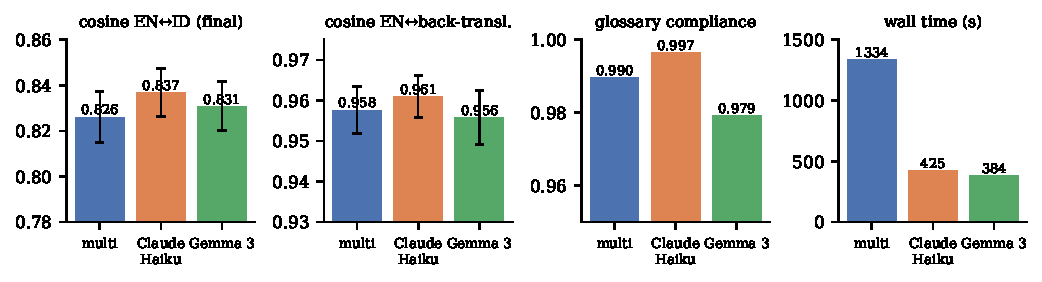
\includegraphics[width=0.95\textwidth]{fig2_configs.pdf}
  \caption{Experiment B: final-text quality (cosine with standard error), glossary compliance and wall time of the three configurations.}
  \label{fig:configs}
\end{figure*}

\paragraph{What the post-editor did}
In \textsc{multi} the post-editor changed 38 of 146 units (26\%); the mean edit ratio over all units is 0.017, and over changed units 0.067 (maximum 0.625). The QA selection kept the reviewed text for 139 units and the draft for 7 (Fig.~\ref{fig:review}a); the two candidates lie close to the diagonal, i.e.\ post-editing rarely changed the automatic score. The change notes describe terminology and grammar corrections: \emph{inferred} rendered as ``diturunkan'' (derived) was corrected to ``disimpulkan''; \emph{show} rendered as ``dibuktikan'' (proven) to ``ditunjukkan''; a hyphenated calque ``sembilan-aturan'' to ``dengan sembilan aturan''; and one complete English sentence that the drafting model had left untranslated in the opening paragraph was translated. None of these is visible in the mean cosine.

\begin{figure*}[t]
  \centering
  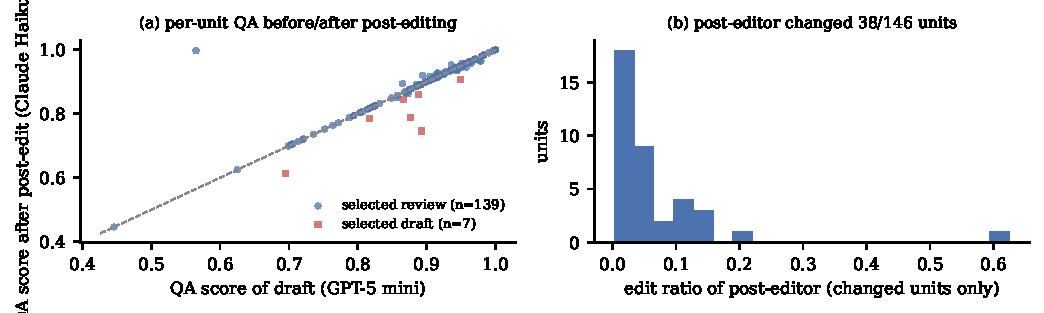
\includegraphics[width=0.95\textwidth]{fig3_review.pdf}
  \caption{\textsc{multi} pipeline: (a) per-unit QA score of the draft and of the post-edited text with the selected candidate; (b) distribution of the post-editor's edit ratio over the 38 changed units.}
  \label{fig:review}
\end{figure*}

\subsection{Experiment C: Who Caught Which Error}
Table~\ref{tab:errors} classifies the errors we found by the layer that caught them. Three classes were caught by validators and by nothing else. (i) \emph{Moved placeholder}: in a pilot run the post-editor, while ``tidying'' number formats, moved the placeholder for \verb|\%| in front of the number (``hanya \ph{3}58'' for ``only 58\%''); the multiset check passed, so the number-gluing rule was added and now rejects such output. (ii) \emph{Echoed back-translation}: on 37 calls for short units (33 post-edited and 4 draft candidates) the local QA model returned the Indonesian text unchanged instead of English; because the back-translation then equalled the candidate, the back-translation cosine collapsed (19 units dropped by more than 0.10) and the selector wrongly preferred the draft for 25 units whose two candidates were identical. The echo rule turns these into failed calls that are retried, after which the selection became 139/7. (iii) \emph{Dropped placeholders}: the local model as sole translator lost placeholders in two paragraphs despite retries; without a fallback model these stay in English and are reported, which is the correct behaviour. Errors caught by a model were semantic: an untranslated sentence, wrong technical terms (\emph{confounder} became ``perusak'' (destroyer) in the local run and ``perancu'' or ``konfonder'' elsewhere; ``stokhastisitas'' misspelled), a table cell ``Union'' left in English and a heading truncated to ``Kritikus lintas'' in the single-Haiku run---the last three were found by human reading, which remains the final layer.

\begin{table}[t]
  \caption{Experiment C: error classes and the layer that caught them (P = post-editing model, Q = QA model, V = deterministic validator, H = human reading).}
  \label{tab:errors}
  \centering
  \small
  \begin{tabular}{@{}p{4.1cm}cp{2.6cm}@{}}
    \toprule
    Error & Caught by & Occurrences \\
    \midrule
    Placeholder moved before a number & V & 1 unit (pilot) \\
    QA model echoed its input & V & 37 calls \\
    Placeholders dropped (local model) & V & 2 units \\
    Sentence left untranslated & P & 1 unit \\
    Wrong technical term & P, H & 4 terms \\
    Misspelling (``stokhastisitas'') & H & 1 unit \\
    Cell or heading left/truncated & H & 2 units (Haiku) \\
    \bottomrule
  \end{tabular}
\end{table}

\subsection{Answers to the Research Questions}
\textbf{RQ1.} No: a vendor SDK can serve a different model from the requested one without any error, and the only truthful label is the model named in the usage event; the agent records it for every call. \textbf{RQ2.} The three-model pipeline did not raise mean quality---a single strong model matched or exceeded it at a third of the time---and structural integrity was a property of the validators rather than of the pipeline (both Copilot configurations reached 146/146); what the pipeline added was the correction of semantic errors that no metric showed. \textbf{RQ3.} Structural and protocol errors (placeholders, echoes) were caught only by validators; semantic errors were caught by a second model or by a human.

\section{Discussion}
\label{sec:discussion}

\paragraph{Averages versus error catching}
The three configurations are statistically indistinguishable on the automatic metrics, and the single strong model is the cheapest way to reach that level. Had we evaluated only by mean cosine we would have concluded that the multi-model pipeline is wasted effort. The per-unit view says otherwise: structural integrity came from the validators (both Copilot configurations reached 146/146, the local model 144/146), and the pipeline's post-editor fixed semantic errors---an untranslated sentence, three wrong terms---that the metrics do not register because a sentence left in English still embeds close to its source. This matches the observation that the benefit of additional LLM calls depends on where the errors are, not on how many calls are made~\cite{chen2024compound}: for a document in which most units are already translated well, a second model mostly agrees (108 of 146 units unchanged) and earns its cost on the few units it changes.

\paragraph{Validators are the cheapest layer and the only one that saw three error classes}
Moved placeholders, echoed back-translations and dropped placeholders are not detectable by a model that reads fluent text, and the judge model was itself the source of one of them. A set-equality check, a regular expression for number-glued placeholders and a string comparison caught all three at negligible cost. This is the same lesson that motivated the companion system~\cite{arya2026wizard}, where a symbolic rule layer validates LLM output: an LLM-as-a-judge~\cite{zheng2023judge} must itself be judged, and the judge of last resort should be deterministic where the property is formal. It also suggests a design for production use---\emph{selective review}: run one strong model with validators on every unit, and send to a second model only the units that validators or cheap heuristics flag (low cosine, residual source-language function words, missed glossary terms, repeated placeholders). On our data such a filter would route roughly a tenth to a quarter of the units, approaching single-model cost with the pipeline's error catching.

\paragraph{Local models for bulk, API models for the final pass}
The local 27B model was the fastest, has no quota, and reached 97.9\% glossary compliance, but it dropped placeholders in two paragraphs and produced the only outright wrong technical term. In the pipeline it serves where its failure modes are cheap: back-translation for QA (where an echo is detected deterministically) and fallback. Which model fills which role should follow from the account's entitlements and the task's error profile, which is why roles, not model names, are the unit of configuration.

\paragraph{Provenance}
Without reading the usage event, this paper would report Haiku's work as Opus's. The requested model is a configuration value; the served model is an observation, and only observations belong in a scientific record. We recommend that research agents (i) log the served model per call, (ii) label outputs with it, (iii) warn on substitution, and (iv) treat an authentication failure as a health failure rather than as an empty result. Model cards~\cite{mitchell2019modelcards} describe models; the agent must still establish which card applies.

\section{Limitations}
\label{sec:limits}
Each configuration was run once; LLM outputs vary between runs~\cite{arya2026wizard}, and the differences we report between configurations (about 0.01 in cosine) are within that variability. All quality metrics are automatic; cross-lingual cosine and back-translation cosine are proxies that are known to miss terminology and fluency errors~\cite{freitag2021mqm,moon2020roundtrip}, which is exactly where the post-editor acted---a human evaluation by bilingual domain experts is needed to quantify that benefit. One language pair, one document type and one glossary were studied. The comparison confounds model choice with the post-editing role: validators were active in all configurations, so the structural results isolate them, but a post-editing pass by the \emph{same} model as the draft was not tested. The QA model also serves as the fallback model, so a systematic weakness of \texttt{gemma3:27b} would affect two roles. Experiment A concerns one vendor SDK and one account tier at one point in time; the behaviour may change, and other providers may reject unknown models. The two-critic review and the DOCX converter are part of the released agent but were not evaluated here.

\section{Conclusion}
\label{sec:conclusion}
We documented that a vendor SDK can silently serve a different model from the one requested and turned the usage event that reveals it into a provenance mechanism for research agents. Around it we built paper-agent, which routes paper-handling tasks to models by role and validates every model output deterministically. In a controlled comparison on 146 LaTeX units, a three-model pipeline did not beat a single model on mean quality or on structural integrity---both came from the validators---but it corrected semantic errors invisible to the metrics; validators caught three error classes that no model, including the judge, detected. Future work is a human evaluation of the post-editor's corrections, a learned filter for selective review, and extending the served-model provenance to other SDKs. As a final check the agent translated this paper into Indonesian with the same pipeline (122 units, 4{,}140 words; 122/122 units structurally intact; glossary compliance 96.6\%; cosine 0.867 direct and 0.961 back-translation; served models \texttt{gpt-5-mini}, \texttt{claude-haiku-4.5} and \texttt{gemma3:27b}); both versions compile from the same bibliography. The code, the per-unit metrics and both language versions are released at \url{https://github.com/devnolife/paper-agent}.


\bibliographystyle{IEEEtran}
\bibliography{references}

\end{document}
